\section{Referencial}\label{sec:refteo}

Este capítulo apresentará a base da literatura que foi coletada durante a preparação desta dissertação, embora os resultados sejam um pouco menores que os de uma tese, eles ainda são relevantes para o trabalho aqui realizado.


     

\subsection{Detec\c c\~ao de anomalias} \label{subsec:detec}



A detecção de anomalias em séries temporais representa um desafio significativo para os previsores, pois requer habilidade em identificar mudanças nos dados, mesmo quando não estão claramente evidentes. Nesse contexto, a coleta de dados realizada ao longo do tempo pela empresa SANEPAR revela anomalias mais expressivas do que inicialmente imaginado. A escassez de água que afetou a cidade de Curitiba se prolongou por vários dias, como é evidenciado pelos gráficos de linha utilizados na etapa de trabalho mencionada (\ref{etp:1}). Esses gráficos oferecem uma representação visual clara das variações nos níveis de água ao longo do tempo, auxiliando na compreensão da extensão do problema e na necessidade de uma abordagem adequada.

\begin{figure}[htp!]
	\centering
	\caption{Dados completos com uma frequência média de 24 horas}
	\label{fig:dados-todos}
	\includegraphics[width=0.9\linewidth]{"Introducao/Figuras/dados todos"}
	
	\fonte{Elaboração própria a partir de dados da SANEPAR (2018 a 2020)}
\end{figure}

\begin{figure}[htp!]
	\centering
	\caption{Plotagem de dados para o ano de 2020}
	\label{fig:2020-a-frente}
	\includegraphics[width=0.9\linewidth]{"Introducao/Figuras/2020 a frente"}
	
	\fonte{Elaboração própria a partir de dados da SANEPAR (2018 a 2020)}
\end{figure}



As Figuras \ref{fig:dados-todos} e \ref{fig:2020-a-frente} apresentadas ilustram visualmente as variações e padrões observados nos dados ao longo do tempo, destacando a importância de explorá-los de maneira apropriada a fim de compreender as anomalias e embasar a tomada de decisões. Os dados coletados possuem uma dimensão de $26.306$ linhas e $9$ colunas, e essa ampla quantidade de dados será utilizada nos modelos descritos na subseção mencionada para que seja possível prever e analisar as anomalias evidenciadas. Essas análises permitirão uma melhor compreensão das anomalias e orientarão as decisões tomadas.








\subsection{Revis\~ao sistem\'atica da literatura} \label{subsec:revisão}

As séries temporais aparecem em vários campos do conhecimento, tais como Economia (preços de estoque diários, taxa de desemprego mensal, produção industrial), Medicina (eletrocardiograma, eletroencefalograma), Epidemiologia (número mensal de novos casos de meningite), Meteorologia (chuvas, temperatura diária, velocidade do vento), etc. Ao longo dos anos tem usado ferramentas computacionais para tornar esta previsão mais eficiente, com aprendizagem de máquinas e algumas características que podem ser aplicadas em linguagem computacional através da linguagem \textit{python e R}, as melhores linguagens para trabalhar com séries temporais hoje em dia.

Para entender melhor este conceito de série temporal, suponhamos que um maratonista que esteja correndo há vários anos e uma pessoa sedentária se submeta a uma corrida de, no máximo, $5$ km, ambos corram ao mesmo tempo para que tenham um monitor de frequência cardíaca para que possa ser monitorado por um médico se você pegar os dados desde o início e compará-los com o final da corrida, o maratonista terá uma série mais estacionária porque ele tem o hábito de correr regularmente enquanto a pessoa sedentária terá uma série não estacionária como mostrado na Figura \ref{fig:series}.


\begin{figure}[H]
	\centering
	\caption{Exemplo de séries temporais}
	\label{fig:series}
	\includegraphics[width=0.9\linewidth]{Revisao/Figuras/séries}
	
	Fonte: \cite{brandão_2020}
\end{figure}


Na figura \ref{fig:series} observa-se que o eixo $x$ representa os dados observados e $t$ para o tempo percorrido.
Além disso, as séries temporais são processos estocásticos por leis probabilísticas, o que significa que há a possibilidade de ser pensado como um conjunto de todas as trajetórias possíveis na Figura \ref{fig:series} é capaz de ser observado para uma variável alvo. Por exemplo, se você lançar um dado qualquer valor inteiro entre 1 e 6, mas apenas um número ocorrerá. Da mesma forma, em séries temporais existem infinitas possibilidades, entre elas apenas uma de acordo com as características que atenderam a esse período e que de fato ocorrerão.

\begin{figure}[H]
	\centering
	\caption{Processo estocástico}
	\label{fig:serie}
	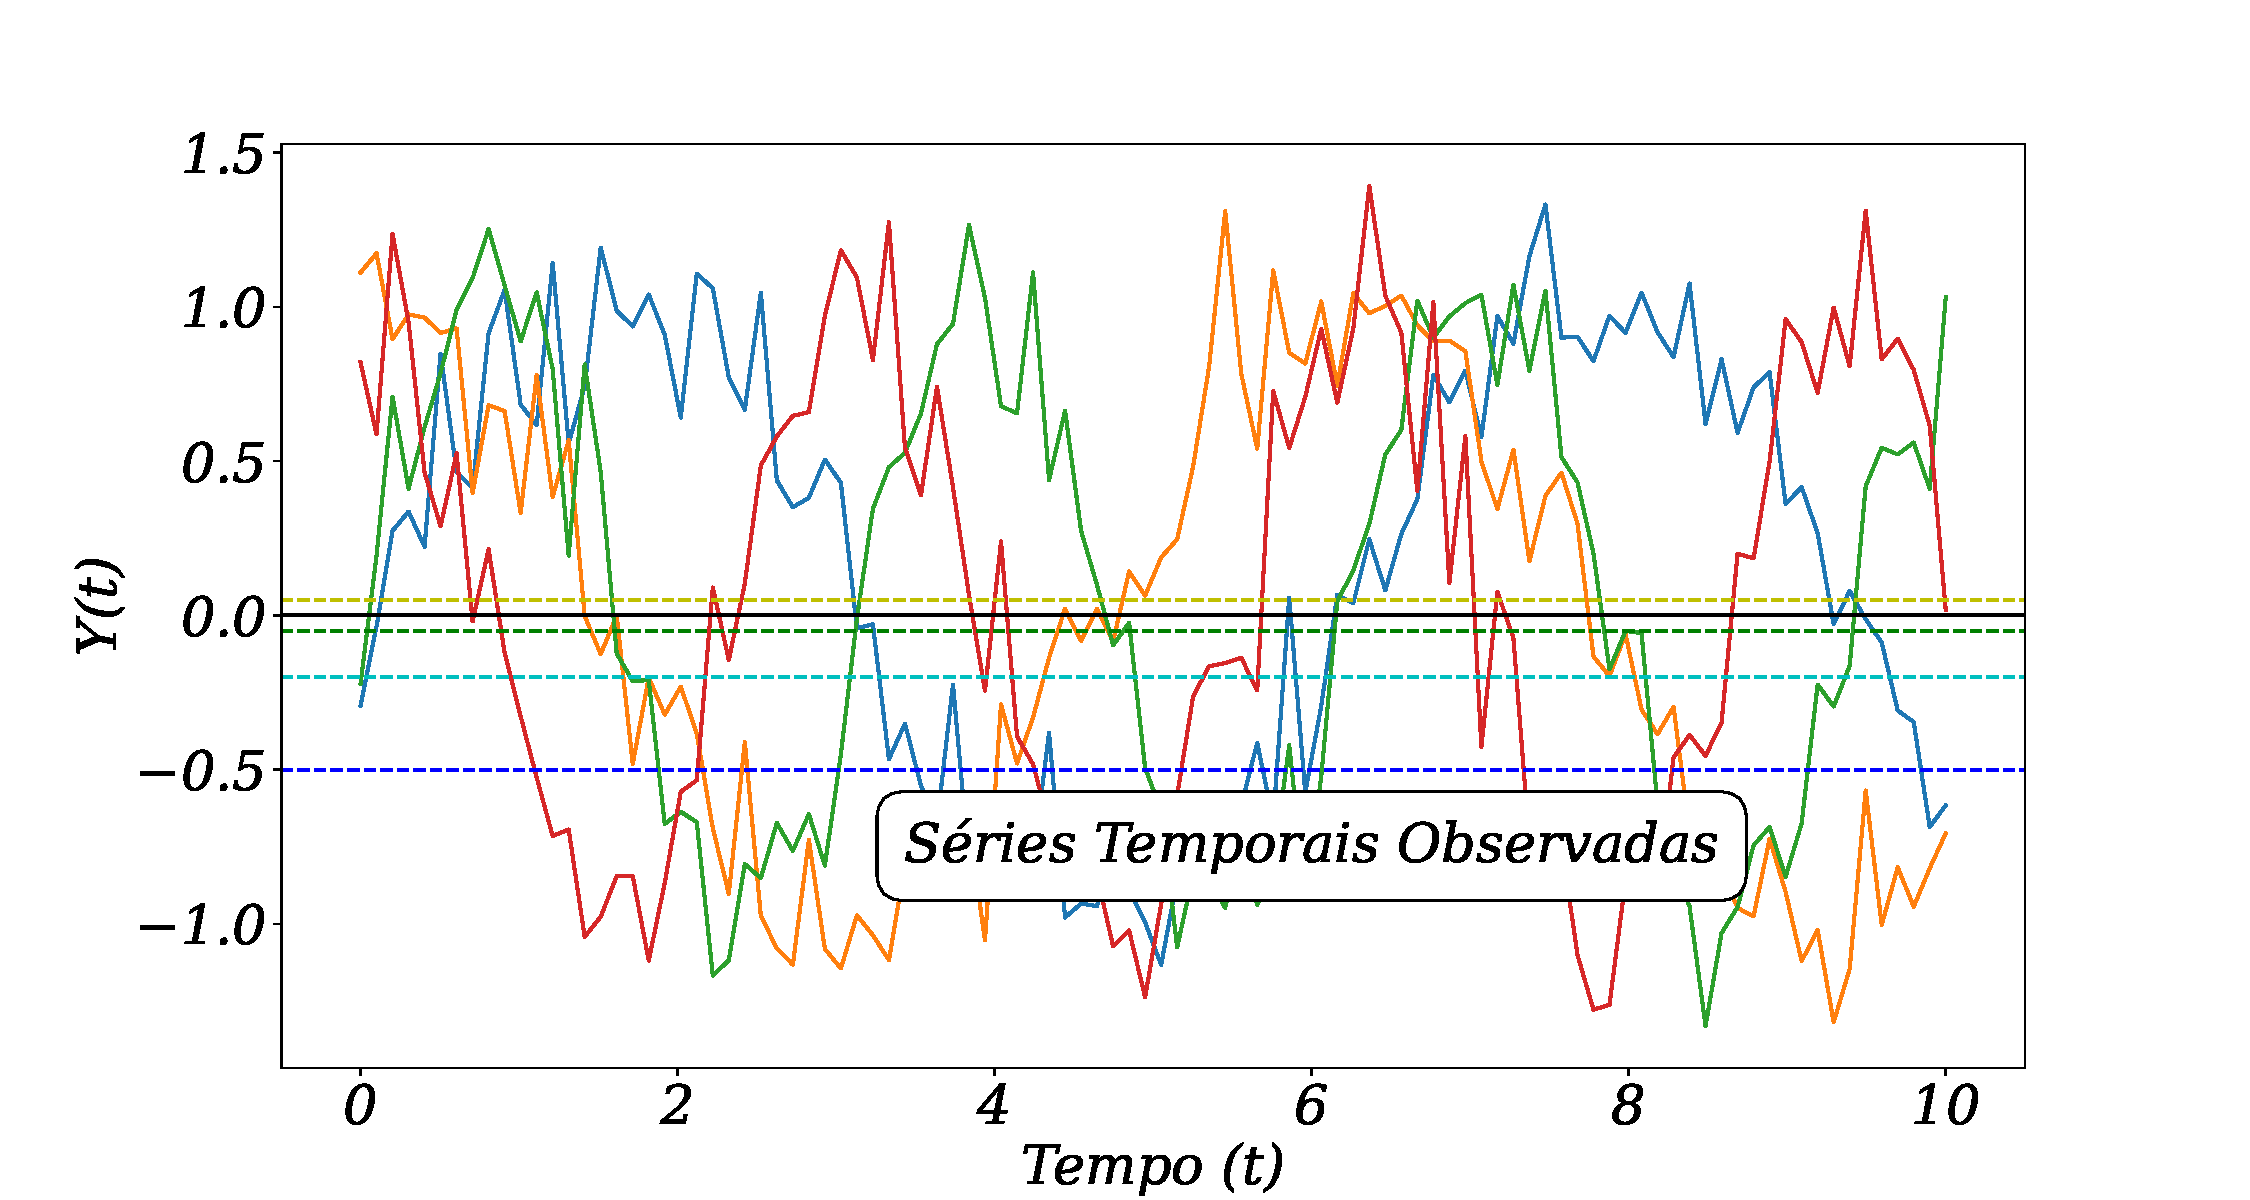
\includegraphics[width=1\linewidth]{Revisao/Figuras/serie}
	
	Fonte: \cite{pinheiro_2022}
\end{figure}

Com $Y(t)$ os dados fictícios e $Tempo \ (t)$ a linha do tempo da Figura \ref{fig:series}.

De repente é pensado como um conjunto de todas as trajetórias possíveis que poderiam ser para observar uma variável.


Esta revisão sistemática da literatura, com o tema abordado até agora é sobre séries temporais, considerando o contexto aqui exposto este tema pode ser de grande relevância em diversas áreas, como mostrado na Figura \ref{fig:areas}. Realizando esta análise de séries temporais nos últimos 6 anos para poder observar as melhores realizações neste tema abordado aqui um curto período, mas tendo o tempo não muito a favor, então teve a opção de deixar este tempo específico para buscar artigos.

O objetivo desta revisão é analisar uma literatura menor, mas muito relevante. Como a própria série temporal procura analisar e modelar a dependência e considerando a ordem apresentada nas bases, por exemplo, os maiores autores e o ano de atividade que mais publicaram nos países que têm o maior número de publicações na apresentação das palavras-chave que serão mostradas, o objetivo é rever cada coisa que pode ser usada em uma aplicação de aprendizagem de máquina.

Em todos os artigos observados que tem uma contribuição científica neste trabalho é a análise do conceito de série temporal com o melhor uso das palavras-chave mesmo não tendo uma grande relação na aprendizagem de máquinas podem ser usados estes artigos como base para outros pesquisadores, aqui algumas análises muito simples para alguns leitores. Entretanto, é um ponto de partida para muitos que não conhecem o conceito de séries cronológicas ou revisão sistemática da literatura.


\subsection{Problematiza\c c\~ao da Revis\~ao} \label{subsec: problematização da revisão}

Nesta seção é abordado um problema de pesquisa que pode ser compreendido por vários leitores na Figura \ref{fig:time-series} é apresentado um mapa conceitual de publicação e os autores são o pilar mais relevante para a revisão porque apresentam vários modelos que servirão de base e como se trata de séries temporais a previsão que pode ser feita neste contexto é um problema de grande significado em si mesmo.

\begin{figure}[H]
	\centering
	\caption{Mapa conceitual do problema de pesquisa}
	\label{fig:serie-temporal}
	\includegraphics[width=1\linewidth]{Revisao/Figuras/"Série temporal"}
	
	Fonte: Elaboração própria 
\end{figure}

No mapa conceitual apresentado na Figura \ref{fig:serial-temporal} é visto o problema sendo relacionado com palavras, tornando evidente o que será abordado durante o trabalho, deixando as questões de pesquisa em tópicos logo à frente.

\begin{enumerate}[start=1, label = {\textbf{Q} \arabic* } ]
	\item \label{questão:rev1}Quais os autores que mais publicam sobre o assunto de séries temporais?
	\item \label{questão:rev2}Quais os países que mais publicam sobre o assunto? 
	\item \label{questão:rev3}Quais as áreas que mais publicam sobre o tema?
	\item \label{questão:rev4}Quais são as obras mais influentes na análise de séries temporais?
\end{enumerate}

\subsection{Metodologia}\label{subsec:met da revisão}

Nesta seção é esclarecido como a revisão foi conduzida desde a análise do banco de dados até a conclusão da revisão.

\begin{figure}[H]
	\centering
	\caption{Etapas da Revisão.}
	\label{fig:rsl}
	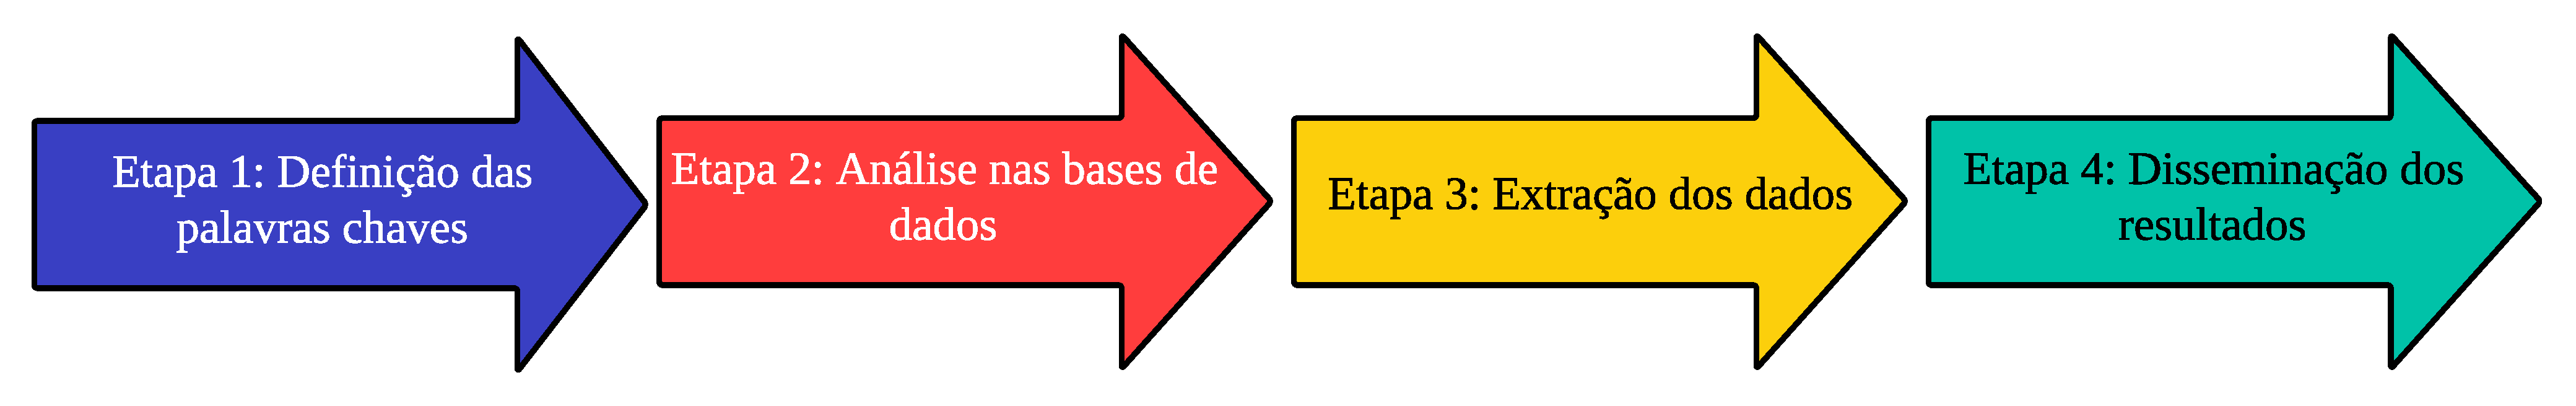
\includegraphics[width=0.7\linewidth]{Revisao/Figuras/RSL}
	
	Fonte: Adaptado de \citeonline{MARTINS201671}
\end{figure}
\begin{enumerate}[start=1, label = {\textbf{Etapa} \arabic* } ]
	
	
\item \label{etp:rev-1}A Figura \ref{fig:rsl} usa uma adaptação de \citeonline{MARTINS201671} para esta revisão sistemática que está sendo analisada. Depois, há as buscas nos bancos de dados Scopus, Web of Science e Lens. No início foram utilizadas algumas bases no meio de tantas na literatura para melhor atender ao tema da pesquisa.


\textbf{Campo de pesquisa Scopus}

\textbf{\textit{TITLE-ABS-KEY (``time series forecasting")  AND  TITLE-ABS-KEY (``time series analysis")  AND  ( LIMIT-TO ( DOCTYPE ,  ``ar" ) )  AND  ( LIMIT-TO ( LANGUAGE ,  ``English" ) )  AND  ( LIMIT-TO ( PUBYEAR ,  2022 )  OR LIMIT-TO ( PUBYEAR ,  2021 )  OR  LIMIT-TO ( PUBYEAR ,  2020 )  OR  LIMIT-TO ( PUBYEAR ,  2019 )  OR  LIMIT-TO ( PUBYEAR ,  2018 )  OR  LIMIT-TO ( PUBYEAR ,  2017 ) )}}

\textbf{Campo de pesquisa na Web of Science}

\textit{\textbf{``times series forecasting" (All Fields) and ``time series analysis" (All Fields)}} (Publication Years: 2022 or 2021 or 2020 or 2019 or 2018 or 2017) (Document Types: Articles) (Languages: English)

\textbf{Campo de pesquisa de Lens}

\textit{\textbf{Scholarly Works (11) = ( ``time series forecasting" ) AND ( ( ``time series analysis" ) AND ( ``nonlinear forecasting" ) ) }}
Filters: Year Published = ( 2016 - 2022  ) Publication Type = ( journal article  )\\

Em todos os campos de busca, foram utilizados os últimos 6 anos, com exceção do site do Lens, onde optamos por 6 anos porque ele devolvia poucos artigos. Nesta etapa, usamos as palavras-chave que melhor se adaptam à busca \textit{time series forecasting and time series analysis and nonlinear forecasting}.


\item \label{etp:rev-2} No cruzamento de palavras obtém-se um número considerável de artigos sem restringir a área em que cada artigo pode ser publicado. Na Tabela \ref{tb1} foi feita uma tabulação dos resultados obtidos sem excluir a duplicata que trataremos na seção \ref{subesec:resul da revisão}.

\item \label{etp:rev-3}Esta etapa é avaliar cada dado obtido sem nenhum filtro no início da busca, a extração destes dados sem utilizar nenhum filtro anual nas buscas seria muitos artigos para analisar, por exemplo, no banco de dados Scopus seria com artigos de $498$, na Web of Sceince seria com artigos de $140$, e na Lente como não retorna muitos artigos é com $11$ dando um total de $649$ sem remover duplicata. É correto lembrar que estes artigos têm apenas o filtro da língua inglesa e do artigo, para melhorar a busca e a tomada de decisão usando o filtro dos anos, os últimos 6 anos é um valor mais agradável de artigos para usar com pouco tempo para analisar, e usando a diferença entre esta estimativa que foi feita na Tabela \ref{tb1} são menos de $356$ artigos para analisar. Lembrando que se a remoção de duplicatas foi feita, este número que foi obtido no resultado de todas as bases pode atingir um número ainda menor do que o pretendido neste trabalho.

\item  \label{etp:rev-4}Nesta etapa é mais analisar a dimensão do que está sendo trabalhado, fazendo a análise das áreas e lendo os artigos que são realmente importantes para a revisão. Como esta revisão está focada em séries temporais em um programa mestre de engenharia de produção e sistemas, vale a pena analisar a correlação. Desta forma, uma das áreas é a matemática, por isso foi selecionada nestes artigos que uma análise mais profunda dos artigos das séries temporais pode resultar se olharmos as áreas de especialização dos artigos pesquisados, como pode ser visto na Figura \ref{fig: áreas} que as áreas aqui citadas com grande relevância são \textbf{informática, engenharia e matemática} tem um número muito alto de publicações representando $50\%$ da pesquisa, então a pesquisa está no caminho certo usando matemática básica para ter uma estimativa de quantos artigos podem ser eliminados seria cerca de $481$ artigos, mas isto sem muita base que este número tem uma precisão. Usando o \textit{software mendeley desktop} para estipular o valor exato de quantos artigos podem ser usados sem duplicação é deixado com um número de artigos de $308$.
\end{enumerate}

\subsection{Resultados da busca de revis\~ao}\label{subesec:resul da revisão}


Nesta seção serão apresentados os resultados da pesquisa utilizando algum software, a fim de estipular o melhor uso de cada banco de dados utilizado durante o trabalho. Assim, pode-se começar com a análise no \textit{software VOSviewer}. 

\begin{figure}[htp!]
	\centering
	\caption{Palavras-chave mais populares na Scopus.}
	\label{fig:scopus-09-08}
	\includegraphics[width=0.9\linewidth]{Revisao/Figuras/"scopus 09-08"}
	
	\vspace{0.2cm}
	Fonte: Elaboração própria a partir de dados da Scopus (2016 a 2022)
\end{figure}
Na figura \ref{fig:scopus-09-08} há uma lista das palavras mais usadas como sinônimos da palavra \textit{time series analysis} ou juntas no corpo do texto dos artigos.
A análise da base de dados no scopus foi feita na ferramenta que mostra as palavras-chave que podem ser relacionadas em cada campo de busca, com isto tem uma visão ampla do que pode ter correlação com as palavras-chave mãe da busca.

Na relação entre as palavras-chave neste primeiro momento, foi obtido um resultado de 3484 palavras-chave, 212 atingindo o limite, lembrando que as palavras base a partir das quais se deve chegar ao texto \textit{``time series forecasting and time series analysis''} em Scopus.



\begin{figure}[htpb!]
	\centering
	\caption{Palavras-chave mais populares na Web of Science}
	\label{fig:web-09-08}
	\includegraphics[width=0.8\linewidth]{Revisao/Figuras/"web 09-08"}
	
	
	
	\fonte{Elaboração própria a partir de dados da Web of Science (2016 a 2022)}
\end{figure}


Na Figura \ref{fig:web-09-08} a análise do banco de dados Web of Science foi feita na ferramenta que mostra as palavras-chave que estão relacionadas em cada campo de busca, com isto você pode ter uma visão ampla do que tem correlação com as palavras-chave mãe da busca.

Na relação entre as palavras-chave neste primeiro momento, teve um resultado de 305 palavras-chave, 13 atingem o limite, lembrando que as palavras base para o resultado foi \textit{``time series forecasting and time series analysis''} na web of science.

O único banco de dados que não será mostrado aqui é o banco de dados Lente, porque é um excelente banco de dados e ainda não retornou muito na busca que foi feita. O site do lens retornou apenas 11 artigos com os filtros aplicados. Na \ref{etp:rev-1} é observado o campo de busca que foi usado nesta busca que deu apenas 11 artigos.



\begin{table}[htpb!]
	\caption{Cruzamento de palavras-chave através da aplicação de filtros de ano e de linguagem}\label{tb1}
	\centering
	\begin{tabular}{@{}cp{2cm}p{1cm}p{2cm}p{1cm}p{2cm}p{2cm}p{2cm}@{}}
		\toprule
		Bases                             & \multicolumn{5}{c}{Palavras Chaves}                                                         & Resultado \\ \midrule
		\multirow{2}{*}{Scopus}           & time   series forecasting & AND & time   series analysis    &     &                         & 490       \\
		& nonlinear forecasting     & AND & time   series forecasting &     &                         & 8         \\
		\multirow{2}{*}{Web   of Science} & time   series forecasting & AND & time   series analysis    &     &                         & 126       \\
		& nonlinear forecasting     & AND & time   series forecasting &     &                         & 14        \\
		Lens                              & time   series forecasting & AND & time   series analysis    & AND & nonlinear   forecasting & 11        \\
		\multicolumn{6}{c}{Total}                                                                                                       & 649       \\ \bottomrule
	\end{tabular}
	
	\fonte{Elaboração própria a partir de dados da Scopus, Lens e Web of Science (2016 a 2022)}
\end{table}


Na Tabela \ref{tb1}, ela lista as palavras-chave para cada base e aumenta a quantidade de artigo em todas as bases, mas esta tabela está com os dados brutos que não foram eliminados as duplicatas, portanto, usando o \textit{software mendeley} para remover as duplicatas devolve apenas 308 artigos.




\begin{figure}[htp!]
	\centering
	\caption{Analise das quantidades de artigos em relação aos anos.}
	\label{fig:regressao-linear-dos-artigos-baseados-nos-anos}
	\includegraphics[width=0.9\linewidth]{Revisao/Figuras/"regressão linear dos artigos baseados nos anos"}
	
	\fonte{Elaboração própria a partir de dados da SANEPAR (2018 a 2020)}
\end{figure}

A figura \ref{fig:regressao-linear-dos-artigos-baseados-nos-anos} tem com abcissas e ordenadas anos e artigos, assim a relação entre a data de publicação dos artigos ao longo do tempo.

Um número considerável de artigos para analisar na Figura \ref{fig:regressao-linear-dos-artigos-baseados-nos-anos} uma análise foi feita com base em uma regressão linear dos artigos ao longo dos anos de 2016 a 2022, nesta análise obteve a seguinte equação de regressão linear:


\begin{eqnarray}
	y(x)&=&8,3571x - 16803 \qquad \text{Com } R^2=0,3062\label{eq1}
\end{eqnarray}

Com $y(x)$ a equação da reta na equação \eqref{eq1}. $8,3571$ é o coeficiente angular do gráfico de $ y(x)$, $16,803$ é o coeficiente linear, ou o ponto de intersecção com o eixo $y$, $x$ é a variável independente.

Este coeficiente indica a proporção da variância da variável dependente que pode ser atribuída estatisticamente ao conhecimento de uma ou mais variáveis independentes \citeonline{coeficiente}. 

O coeficiente de determinação mede a relação que existe entre a variável dependente e as variáveis independentes, indicando que porcentagem da variação explicada pela regressão representa da variação total. Quando:

$R^2=1$: todos os pontos observados estão exatamente na reta de regressão (ajuste perfeito), ou seja, as variações de $y$ são de $100\%$ explicadas pela variação de $x_n$ através da função especificada, sem desvios em torno da função estimada. 

$R^2=0$: conclui-se que as variações de $y$ são exclusivamente aleatórias e a introdução das variáveis $x_n$ no modelo não incorporará nenhuma informação sobre as variações de $y$.

\begin{equation}
	R^{2}=\frac{\left(\sum X . Y-\frac{\sum X \cdot \sum Y}{n}\right)^{2}}{\left[\sum X^{2}-\frac{\left(\sum X\right)^{2}}{n}\right] \cdot\left[\sum Y^{2}-\frac{\left(\sum Y\right)^{2}}{n}\right]}=(r)^{2}\label{eq2}
\end{equation}

Na equação \eqref{eq2} $X,Y$ é dado pelas coordenadas no plano cartesiano como por exemplo o par encomendado $(x,y)$. 
Na equação \eqref{eq1} observa-se que obteve o $R^2=30\%$ isto implica que a linha de regressão será influenciada pelo $R^2$ que foi encontrado.

Embora seja uma análise muito simples que foi realizada com a relação entre número de artigos e anos, ainda é uma validação muito boa para olhar para o teste F de significância que é dado o significado tem que ser sempre $F<5\%$ este teste também é chamado de p-valor.

Tendo estes valores, é possível analisar o significado extremo da linha de regressão e observar que 2021 foi o ano em que a maioria dos artigos foram publicados sobre este tema da séries temporais.

\begin{table}[H]
	\centering
	\caption{Fator de impacto}\label{tb2}
	\begin{tabular}{@{}cp{3cm}p{3cm}c@{}}
		\toprule
		Revista cientíica      & Quantidade de plubicação & Qualidade da revista & H-INDEX \\\midrule
		Neurocomputing         & 27                         & Q1                     & 143     \\
		IEEE Access            & 18                         & Q1                     & 127     \\
		Applied Soft Computing & 12                         & Q1                     & 143     \\
		Energies               & 11                         & Q2                     & 93      \\
		Energy                 & 11                         & Q1                     & 343     \\ \bottomrule
	\end{tabular}
	
	
	\fonte{Elaboração própria a partir de dados da Scopus, Lens e Web of Science (2016 a 2022)}
\end{table}

Na Tabela \ref{tb2} mostra revistas que a maioria publica artigos sobre este assunto, já que muitas revistas não estão localizadas no Brasil e têm seus nomes em inglês, mas todas as revistas com um fator de impacto muito alto como \textbf{A1} têm uma correlação com as áreas de \textbf{informática, engenharia e matemática}.

\begin{figure}[htpb!]
	\centering
	\caption{Relação de autores entre artigos publicados}
	\label{fig:autores-relacao-entre-artigos-publicados}
	\includegraphics[width=0.8\linewidth]{Revisao/Figuras/"Autores Relação entre artigos publicados"}
	
	
	\fonte{Elaboração própria a partir de dados da Scopus (2016 a 2022)}
\end{figure}

\begin{figure}[htpb!]
	\centering
	\caption{Ligação bibliográfica entre os autores}
	\label{fig:autores}
	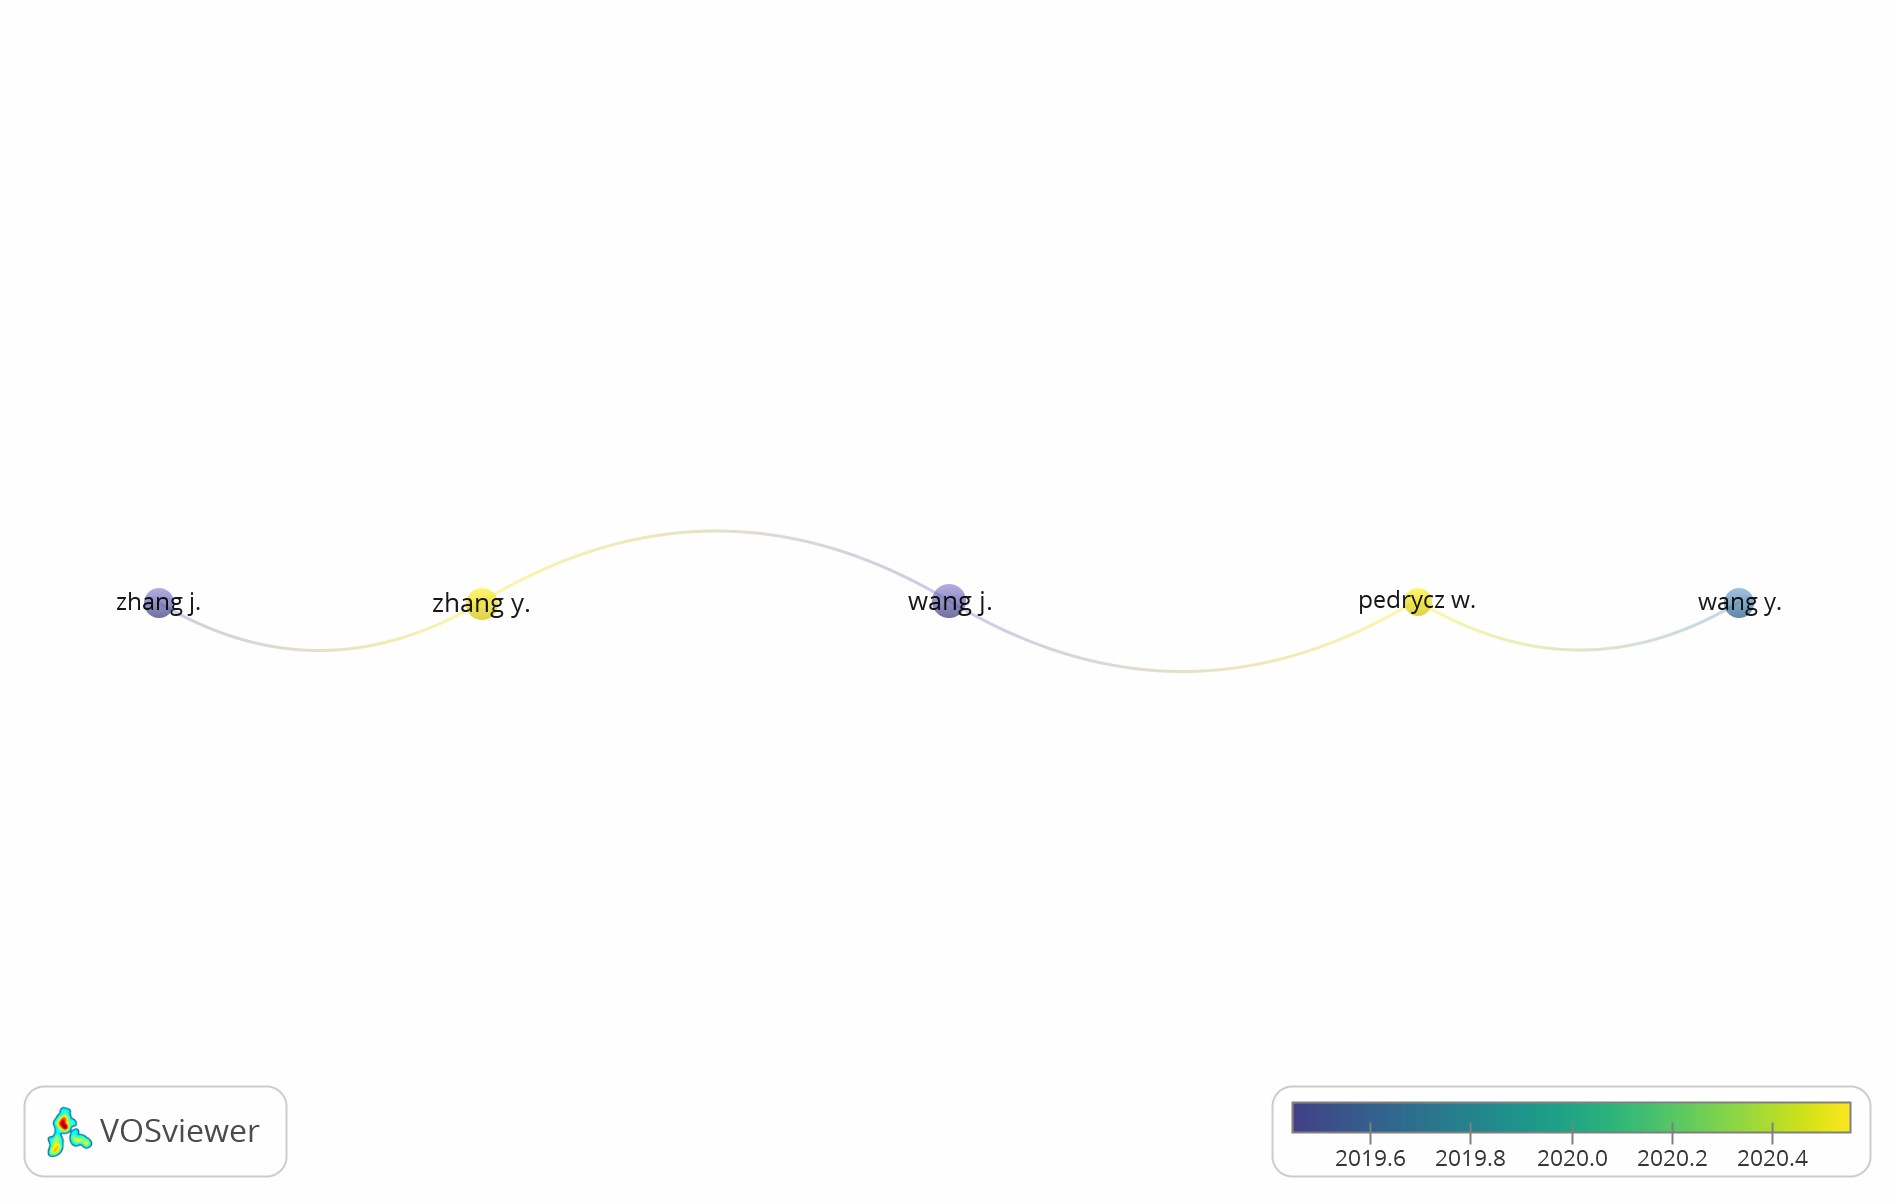
\includegraphics[width=0.8\linewidth]{Revisao/Figuras/Autores}
	
	\fonte{Elaboração própria a partir de dados da Scopus (2016 a 2022)}
\end{figure}

 Respondendo a um problema aqui colocado, o \ref{questão:rev1} usa a Figura \ref{fig:autores-relacao-entre-artigos-publicados} com um gráfico de histograma para ser mais visível que os autores que mais publicaram neste tópico no gráfico colocam os autores que tiveram publicação maior que 4 e com isto não coloca todos os autores considerando os autores que publicaram mais de 4 artigos neste tópico de 2016 a 2022.


\begin{figure}[htpb!]
	\centering
	\caption{Mapa mundial da publicação de artigos em todo o mundo}
	\label{fig:mapa-mundi-artigos}
	\includegraphics[width=1\linewidth]{Revisao/Figuras/"mapa mundi artigos"}
	\vspace{0.2cm}
	
	\fonte{Elaboração própria a partir de dados da Scopus, Lens e Web of Sicence (2016 a 2022)}
\end{figure}

Na pergunta de pesquisa \ref{questão:rev2} é respondido com a Figura \ref{fig:mapa-mundi-artigos} os países que mais público sobre o assunto em escala desde a maior publicação até a menor em escala, como segue China - 119, Estados Unidos - 67, Índia - 57, Brasil - 32, Espanha - 28, Reino Unido - 25, Austrália - 24, Irã - 18, Malásia - 17, Canadá - 16. O mapa não mostra todos os países com seus números de publicação.


\begin{figure}[htpb!]
	\centering
	\caption{Áreas de aplicação do tema}
	\label{fig:areas}
	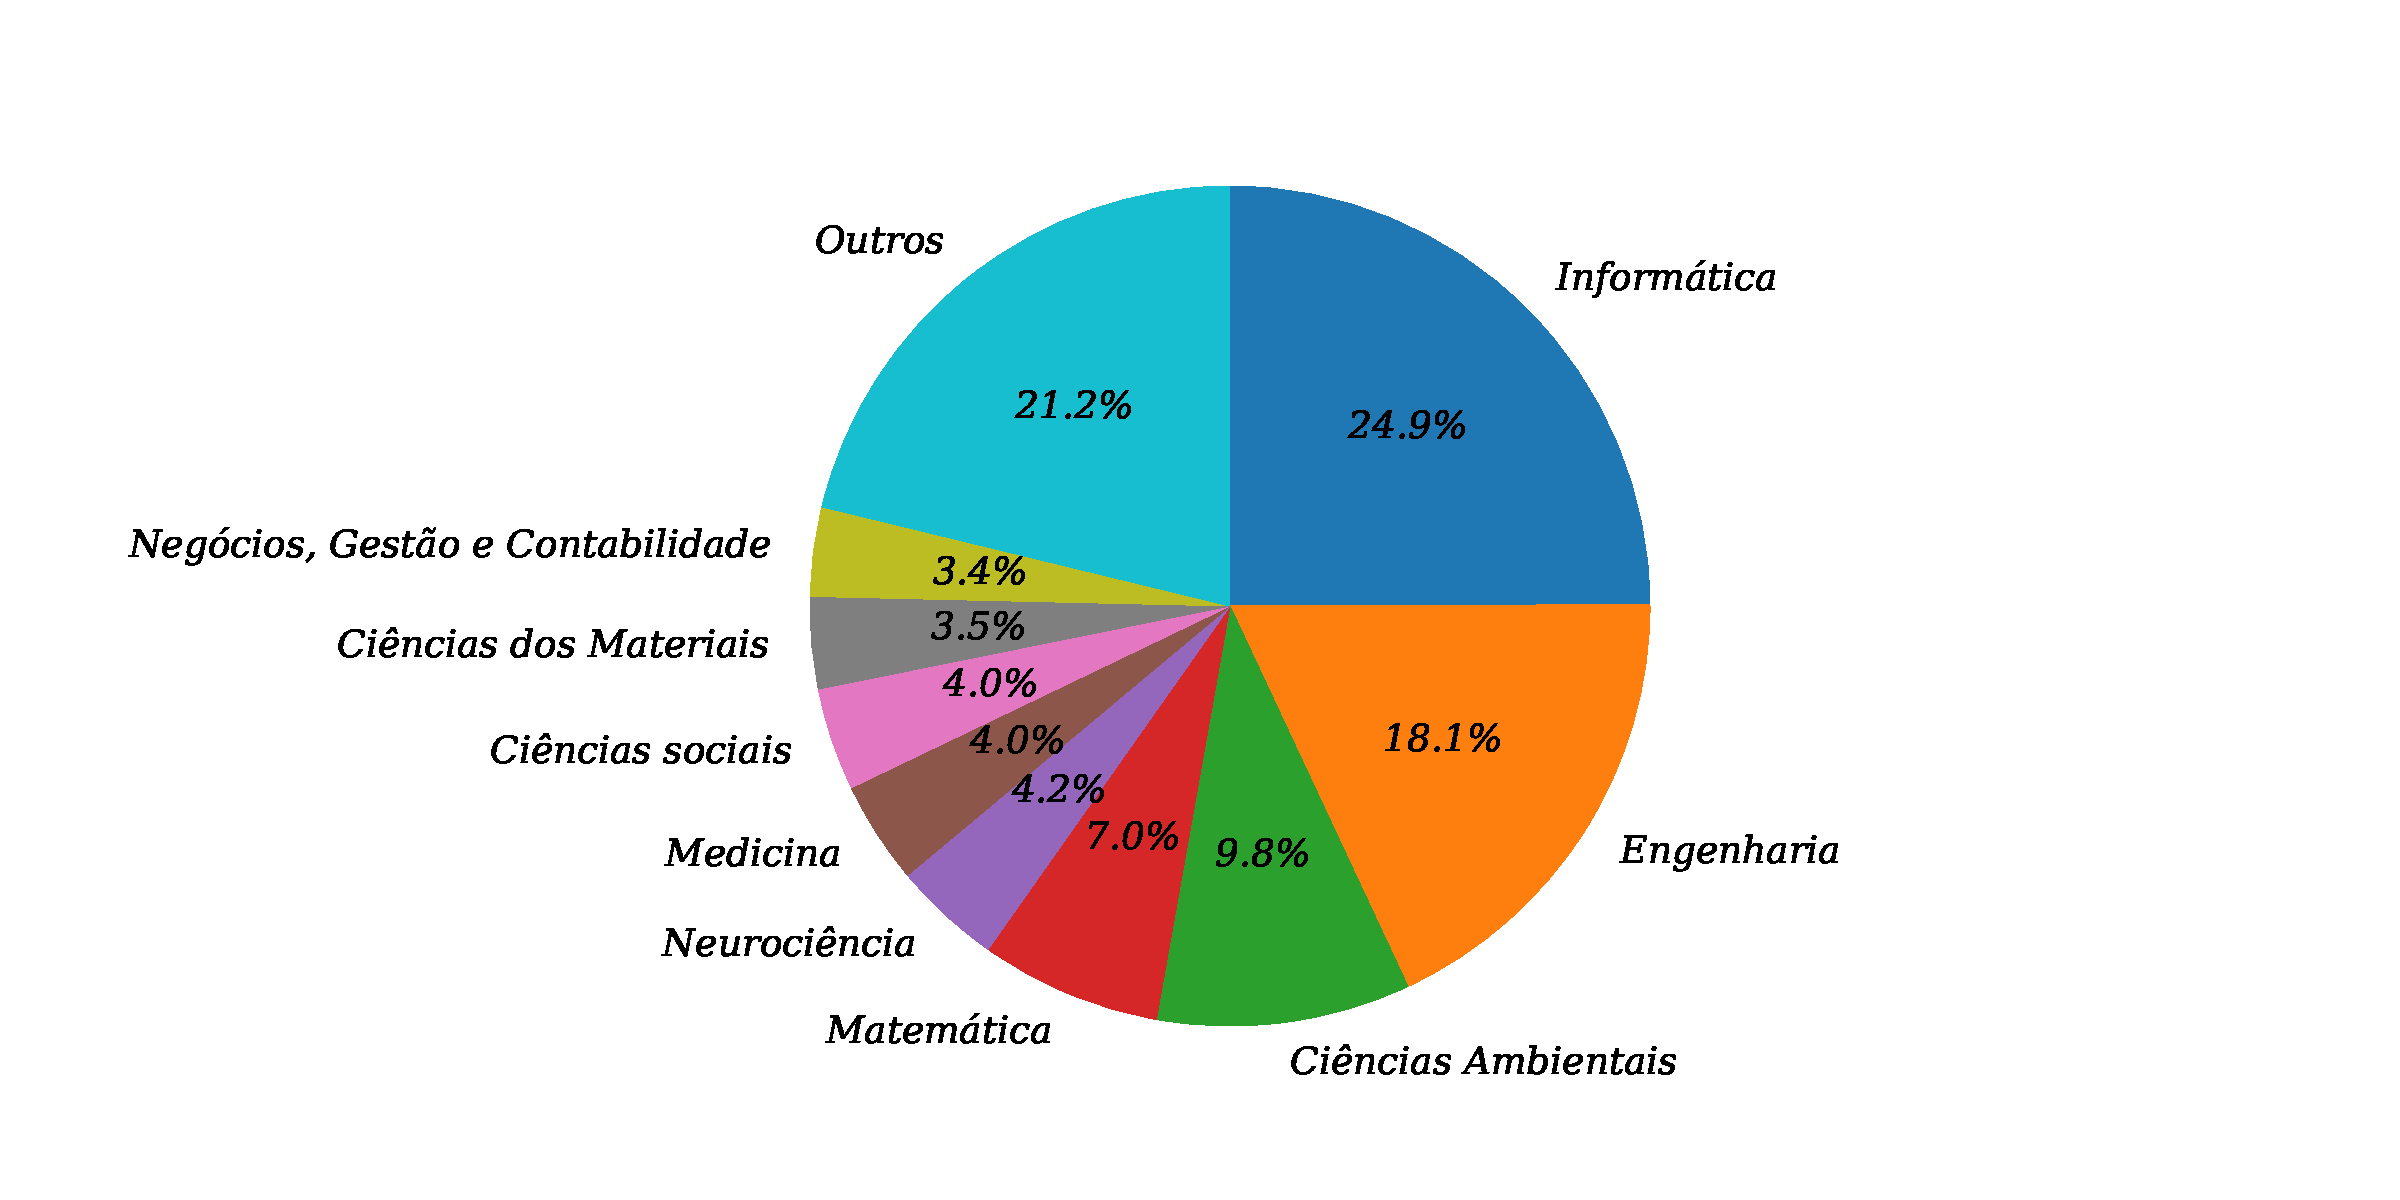
\includegraphics[width=0.9\linewidth]{Revisao/Figuras/areas}
	\vspace{0.2cm}
	
	\fonte{Elaboração própria a partir de dados da Scopus, Lens e Web of Sicence (2016 a 2022)}
\end{figure}


Pergunta de pesquisa \ref{question:rev3} para responder a esta pergunta, foi feito um gráfico circular para rotular as áreas que têm mais publicação no tempo escolhido na revisão. A Tabela \ref{tb3} mostra os valores de cada área e sua quantidade de publicação. 

\begin{table}[!htb]
	\centering
	\caption{Áreas e seus valores respetivos de artigos em cada área.}\label{tb3}
	\begin{tabular}{@{}ll@{}}
		\toprule
		Informática                      & 240 \\ \midrule
		Engenharia                       & 174 \\
		Ciências Ambientais              & 94  \\
		Matemática                       & 67  \\
		Neurociência                     & 40  \\
		Medicina                         & 38  \\
		Ciências sociais                 & 38  \\
		Ciências dos Materias            & 34  \\
		Negócios, Gestão e Contabilidade & 33  \\
		Outros                           & 204 \\ \bottomrule
	\end{tabular}

	
	\fonte{Elaboração própria a partir de dados da Scopus, len e Web of Sicence (2016 a 2022)}
\end{table}
	

Na última pergunta de pesquisa \ref{questão:rev4} foi feita uma pesquisa sobre alguns dos artigos mais influentes na revisão, esses artigos retratam alguns métodos sobre séries temporais dos artigos dos autores \citeonline{Golyandina2020, Kumar2021, Xie2019, Lara-Benitez2021, Ahmad2018, CarvalhoJr.2019, Tan2021, Liu2019, Liu2021, Rossi2018, Soyer, Martinovic2020a, Ursu2016, Wang2016, Shih2019a, Moon2019, Chou2018, Bergmeir2018, Boroojeni2017, Chou2018a, Coelho2017, Du2020, Sadaei2019, Salgotra2020, Tyralis2017, Vlachas2020, Yang2019a, Shen2020, Sezer2020, Chen2018, Buyuksahin2019, Li2020, Kulshreshtha2020, Samanta2020, Xu2019, Graff2017, Taieb2016}
 alguns métodos usados pelos autores para previsão de séries temporais e alguns modelos de análise da mesma previsão não-linear. 

 
\citeonline{Xu2019} no modelo híbrido, o modelo linear AR e LR ou o modelo ARIMA e o modelo DBN não-linear são explorados para capturar os comportamentos lineares e não-lineares de uma série temporal, respectivamente. \citeonline{Li2020} o desempenho de previsão da abordagem MAELS é comparado com os predecessores baseados na aprendizagem de máquinas de última geração como CNN, RNN, LSTM, ARIMA, e SVM-VAR. As abordagens, CNN, RNN e LSTM permitem o manuseio multivariado de entrada e saída, ARIMA usa dados passados para prever o futuro usando duas características principais: autocorrelação e médias móveis.

 
Assim, com esta revisão sistemática e análise de conteúdo, a resposta à pergunta de pesquisa feita no início do capítulo foi obtida.

Fora destes modelos, também há a atualização ARIMA que será utilizada nesta dissertação, pois SARIMA, SARIMAX ambos os modelos serão comparados para se obter o melhor modelo entre eles, fora disto também será utilizado o Light GBM e o XGBoost. Para as métricas de erro nesta dissertação serão utilizadas as seguintes métricas e explicadas no capítulo \ref{sec:base} MAE, MAPE e RMSE na literatura é um dos mais utilizados entre vários com, por exemplo, os $R^2$ citados \eqref{eq2} para as previsões futuras sempre foram confrontados com estas métricas de erro. os $R^2$ não são tão utilizados para comparação.



\subsection{Conclus\~ao da revis\~ao} \label{subsec:conclusão da revisão}

Nesta seção para relatar o que foi coberto durante a pesquisa de revisão sendo ela em algumas bases como Scopus, Web of Science e Lens, cada base retornou vários artigos que foram analisados e assim responde a pergunta de pesquisa feita na revisão apesar de a base de Lens ser a menor de todas ainda encontra alguns artigos que foram relevantes no processo de dissertação também com a ajuda do \textit{software} para analisar muitos arquivos e suas relações entre cada um. Sendo a série temporal uma análise mais profunda e mais atual na revisão sistemática fazendo a pesquisa nos últimos 6 anos.

Na busca realizada foram obtidos alguns resultados muito relevantes, pois no cruzamento das palavras em cada base com o filtro aplicado foram obtidos artigos de $308$ de $2016$ a $2022$, com isso foi necessário filtrar mais sobre cada área de desempenho dos artigos, tais como matemática, engenharia e informática neste filtro tinha um total de artigos de $481$ excluindo que seriam das outras áreas.




